\documentclass[CAT]{TFUOC}%IB: CASTELLÀ, CAT: CATALÀ, ENG: ANGLÈS

%Compatibilitat amb Pandoc
\usepackage[T1]{fontenc}
\usepackage{lmodern}
\usepackage{amsmath,longtable,booktabs,fancyvrb,framed}
\providecommand{\tightlist}{\setlength{\itemsep}{0pt}\setlength{\parskip}{0pt}}
\providecommand{\pandocbounded}[1]{#1}

\usepackage{color}
\usepackage{fancyvrb}
\newcommand{\VerbBar}{|}
\newcommand{\VERB}{\Verb[commandchars=\\\{\}]}
\DefineVerbatimEnvironment{Highlighting}{Verbatim}{commandchars=\\\{\}}
% Add ',fontsize=\small' for more characters per line
\usepackage{framed}
\definecolor{shadecolor}{RGB}{248,248,248}
\newenvironment{Shaded}{\begin{snugshade}}{\end{snugshade}}
\newcommand{\AlertTok}[1]{\textcolor[rgb]{0.94,0.16,0.16}{#1}}
\newcommand{\AnnotationTok}[1]{\textcolor[rgb]{0.56,0.35,0.01}{\textbf{\textit{#1}}}}
\newcommand{\AttributeTok}[1]{\textcolor[rgb]{0.13,0.29,0.53}{#1}}
\newcommand{\BaseNTok}[1]{\textcolor[rgb]{0.00,0.00,0.81}{#1}}
\newcommand{\BuiltInTok}[1]{#1}
\newcommand{\CharTok}[1]{\textcolor[rgb]{0.31,0.60,0.02}{#1}}
\newcommand{\CommentTok}[1]{\textcolor[rgb]{0.56,0.35,0.01}{\textit{#1}}}
\newcommand{\CommentVarTok}[1]{\textcolor[rgb]{0.56,0.35,0.01}{\textbf{\textit{#1}}}}
\newcommand{\ConstantTok}[1]{\textcolor[rgb]{0.56,0.35,0.01}{#1}}
\newcommand{\ControlFlowTok}[1]{\textcolor[rgb]{0.13,0.29,0.53}{\textbf{#1}}}
\newcommand{\DataTypeTok}[1]{\textcolor[rgb]{0.13,0.29,0.53}{#1}}
\newcommand{\DecValTok}[1]{\textcolor[rgb]{0.00,0.00,0.81}{#1}}
\newcommand{\DocumentationTok}[1]{\textcolor[rgb]{0.56,0.35,0.01}{\textbf{\textit{#1}}}}
\newcommand{\ErrorTok}[1]{\textcolor[rgb]{0.64,0.00,0.00}{\textbf{#1}}}
\newcommand{\ExtensionTok}[1]{#1}
\newcommand{\FloatTok}[1]{\textcolor[rgb]{0.00,0.00,0.81}{#1}}
\newcommand{\FunctionTok}[1]{\textcolor[rgb]{0.13,0.29,0.53}{\textbf{#1}}}
\newcommand{\ImportTok}[1]{#1}
\newcommand{\InformationTok}[1]{\textcolor[rgb]{0.56,0.35,0.01}{\textbf{\textit{#1}}}}
\newcommand{\KeywordTok}[1]{\textcolor[rgb]{0.13,0.29,0.53}{\textbf{#1}}}
\newcommand{\NormalTok}[1]{#1}
\newcommand{\OperatorTok}[1]{\textcolor[rgb]{0.81,0.36,0.00}{\textbf{#1}}}
\newcommand{\OtherTok}[1]{\textcolor[rgb]{0.56,0.35,0.01}{#1}}
\newcommand{\PreprocessorTok}[1]{\textcolor[rgb]{0.56,0.35,0.01}{\textit{#1}}}
\newcommand{\RegionMarkerTok}[1]{#1}
\newcommand{\SpecialCharTok}[1]{\textcolor[rgb]{0.81,0.36,0.00}{\textbf{#1}}}
\newcommand{\SpecialStringTok}[1]{\textcolor[rgb]{0.31,0.60,0.02}{#1}}
\newcommand{\StringTok}[1]{\textcolor[rgb]{0.31,0.60,0.02}{#1}}
\newcommand{\VariableTok}[1]{\textcolor[rgb]{0.00,0.00,0.00}{#1}}
\newcommand{\VerbatimStringTok}[1]{\textcolor[rgb]{0.31,0.60,0.02}{#1}}
\newcommand{\WarningTok}[1]{\textcolor[rgb]{0.56,0.35,0.01}{\textbf{\textit{#1}}}}

% Suport per a citacions CSL (Zotero / Pandoc)
\usepackage{calc}

\providecommand{\citeproctext}{}
\newlength{\cslhangindent}
\setlength{\cslhangindent}{1.5em}
\newlength{\csllabelwidth}
\setlength{\csllabelwidth}{2.5em}

\newcommand{\CSLBlock}[1]{#1\hfill\break}
\newcommand{\CSLLeftMargin}[1]{\parbox[t]{\csllabelwidth}{#1}}
\newcommand{\CSLRightMargin}[1]{\parbox[t]{\linewidth - \csllabelwidth}{#1}}
\newcommand{\CSLRightInline}[1]{\parbox[t]{\linewidth - \csllabelwidth}{#1\break}}
\newcommand{\CSLIndent}[1]{\hspace{\cslhangindent}#1}

\newenvironment{CSLReferences}[2] % #1 hanging-indent, #2 entry spacing
 {\begin{list}{}{%
  \setlength{\itemindent}{0pt}%
  \setlength{\leftmargin}{0pt}%
  \setlength{\parsep}{0pt}%
  \setlength{\itemsep}{#2pt}%
  \setlength{\labelwidth}{0pt}%
  \setlength{\labelsep}{0pt}%
  \renewcommand{\makelabel}[1]{}% Buida l'etiqueta de \item per evitar [] o punts
  }}
 {\end{list}}

\usepackage{enumitem}
\usepackage{float}

\usepackage[hidelinks,unicode]{hyperref}


%Introducció de dades del treball
\title{Biaixos de sexe i gènere en rehabilitació cardíaca: anàlisi d'equitat algorítmica (\emph{fairness}) en la predicció de resultats clínics}
\titcrt{\emph{Fairness} en rehabilitació cardíaca} %Títol curt que apareixerà a la capçalera
\author{Guillem Lluís i Luengo}
\date{7 d'octubre de 2026}

\nomPDC{Susana Pérez Álvarez}
\nomPRA{Laia Subirats Maté}
\titulac{Màster Universitari en Bioinformàtica i Bioestadística}
\area{Estudis Clínics i Epidemiològics}
\idioma{Català}
\credits{15}
\parcla{cardiac rehabilitation, machine learning, fairness, clinical outcomes, sex and gender bias}
\licenc{ccBy}


%%%%%%%%%%
% Resum en l'idioma

\abstractidioma{Màxim 250 paraules, amb la finalitat, context d'aplicació, metodologia, resultats i conclusions del treball.}

% Resum en anglès.
\abstractenglish{A maximum of 250 words, detailing the purpose, context of application, methodology, results and conclusions of the work.}

\begin{document}

\estructura

\tableofcontents

\listoffigures

\listoftables

\chapter{Introducció}\label{introducciuxf3}

\section{Context i justificació del treball}\label{context-i-justificaciuxf3-del-treball}

La rehabilitació cardíaca (RC) és una intervenció amb eficàcia demostrada per a la recuperació posterior a esdeveniments cardiovasculars. Les persones que participen en programes de RC presenten millors resultats clínics, a més d'una reducció en la taxa de readmissions hospitalàries i en la mortalitat i d'un efecte positiu en la qualitat de vida {[}1{]}. No obstant això, la participació en aquesta mena d'intervencions és considerablement baixa i existeixen diferències de gènere en tres àrees clau: l'accés als programes, l'adherència al tractament i els resultats clínics obtinguts. Les barreres que originen aquestes desigualtats poden ser individuals, socials o pròpies dels sistemes sanitaris {[}2{]}.

La infrarepresentació de les dones, així com d'altres col·lectius vulnerables, pot conduir a biaixos en la recerca i, en última instància, a una disminució de l'eficàcia dels tractaments. Els mètodes d'aprenentatge automàtic (ML, per les seves sigles en anglès) poden ser útils per mitigar aquestes desigualtats, però també poden perpetuar-les si no se'n tenen en compte els potencials biaixos {[}3{]}. Per això és necessari disposar d'eines per avaluar l'equitat algorítmica (\emph{fairness}) dels models emprats i, posteriorment, millorar-la sense comprometre la precisió de les prediccions.

La tria de l'àmbit del treball està motivada per la meva formació i experiència professional prèvia com a fisioterapeuta, amb especial interès en la rehabilitació cardiorespiratòria. Si bé els biaixos en el diagnòstic i el tractament de patologies cardiovasculars són de domini públic des de fa temps, no s'ha d'oblidar l'impacte que tenen al llarg de tot el procés d'atenció sanitària, en què intervenen altres disciplines a banda de la medicina. És important dur a terme recerca de qualitat en infermeria, fisioteràpia, psicologia o nutrició per assegurar uns resultats òptims i lliures de discriminacions.

En definitiva, aquest treball pretén estudiar l'impacte dels biaixos de sexe i gènere en la predicció de resultats clínics de la RC, avaluar-ne l'equitat algorítmica i proposar mesures per atenuar-ne els efectes.

\section{Descripció general}\label{descripciuxf3-general}

Per a la realització d'aquest treball, s'ha optat per utilitzar l'estudi \emph{Functional capacity and patient-reported outcome measures after cardiac rehabilitation: a prospective study with 6-month follow-up} {[}4{]} com a font de dades. S'hi pot accedir a través dels enllaços que s'inclouen a continuació:

\begin{itemize}
\item
  \textbf{Estudi}: \url{https://smw.ch/index.php/smw/article/view/4160/6376}.
\item
  \textbf{Dades}: \url{https://data.mendeley.com/datasets/hbztb7wmc5/1}.
\end{itemize}

El conjunt de dades conté 273 registres, majoritàriament homes (81\%). Si bé aquest fet pot esdevenir una limitació per a l'auditoria de gènere, també evidencia el biaix de representació existent a la literatura científica. Les variables sobre les quals es treballarà es poden agrupar en tres àmbits:

\begin{itemize}
\item
  \textbf{Demogràfiques}: edat, sexe, diagnòstic, antecedents de tabaquisme.
\item
  \textbf{Capacitat funcional}: test de 6 minuts de marxa (6MWT), capacitat d'exercici màxima a curt termini (MSEC), equivalent metabòlic de la tasca (MET), força isomètrica màxima del quàdriceps (QIS).
\item
  \textbf{Qüestionaris de salut}: escales d'ansietat i depressió (HAD), qualitat de vida (HeartQoL) i nivells de treball, esport i activitat física (Baecke).
\end{itemize}

\section{Objectius del treball}\label{objectius-del-treball}

A continuació es detalla la relació d'objectius principals i secundaris del treball:

\begin{enumerate}[label=\arabic*.]
\item Determinar l'impacte dels biaixos de sexe i gènere en la predicció de la resposta a la rehabilitació cardíaca.

  \begin{enumerate}[label*=\arabic*.]
  \item Descriure l'estat actual de l'evidència científica en l'àmbit d'estudi.
  \item Elaborar diferents models predictius per explicar els resultats de les variables d'interès.
  \item Quantificar les diferències en les prediccions dels models proposats mitjançant mètriques d'equitat algorítmica.
  \end{enumerate}
  
\item Proposar mesures per atenuar els biaixos detectats.

  \begin{enumerate}[label*=\arabic*.]
  \item Exposar tècniques de preprocessament, processament i postprocessament utilitzades per corregir la disparitat de les dades.
  \item Avaluar l'adequació de les mesures als models predictius proposats.
  \end{enumerate}

\end{enumerate}

\section{Enfocament i mètode seguit}\label{enfocament-i-muxe8tode-seguit}

\subsection{Estratègia de recerca}\label{estratuxe8gia-de-recerca}

En una primera fase del treball, es durà a terme una cerca de literatura científica a les principals bases de dades d'investigació clínica (PubMed, Cochrane Library, ScienceDirect\ldots), així com en altres fonts especialitzades que es considerin rellevants.

Els resultats obtinguts es filtraran segons la seva adequació al tema i es classificaran en tres àmbits que permetran estructurar-ne adequadament els continguts:

\begin{itemize}
\item
  \textbf{Rehabilitació cardíaca}: estat de l'art general, càrrega de les patologies cardiovasculars en la salut global, impacte en resultats clínics, descripció de variables predictores {[}5--7{]}.
\item
  \textbf{Biaixos de sexe i gènere}: diferències en l'accés, la participació i els resultats de la rehabilitació cardíaca, interseccionalitat de les desigualtats, intervencions proposades {[}8--12{]}.
\item
  \textbf{Equitat algorítmica}: evidència sobre mètodes estadístics, limitacions i propostes de mitigació de biaixos {[}13--15{]}.
\end{itemize}

\subsection{Metodologia de treball}\label{metodologia-de-treball}

Un cop feta la recerca d'evidència, es procedirà a l'anàlisi de les dades disponibles mitjançant el programari \texttt{R} i adoptant, en la mesura del possible, els principis del \texttt{tidyverse}. Se seguiran els passos que s'indiquen:

\begin{itemize}
\item
  \textbf{Preprocessament de dades}: neteja, tractament de valors nuls, anàlisi descriptiva estratificada per sexe i definició de variables objectiu. Les principals variables d'interès són la capacitat funcional (mesurada habitualment amb el 6MWT) i la qualitat de vida, que es poden binaritzar en funció de si la millora és superior o no a la mínima diferència clínicament important per a cada cas.
\item
  \textbf{Modelització estadística}: construcció de models predictius a partir del conjunt de dades. Tenint en compte les característiques de les variables objectiu, es prendrà com a model de referència la regressió logística. S'optimitzarà el model amb mètodes de regularització (Ridge, LASSO). Malgrat que el nombre de registres és limitat, es podria comparar el resultat amb una alternativa no lineal, com ara un Random Forest.
\item
  \textbf{Avaluació i auditoria de gènere}: valoració del rendiment del model. A més de les mesures habituals, s'utilitzaran les mètriques d'equitat algorítmica que es considerin adequades d'entre les descrites a la literatura científica.
\item
  \textbf{Discussió de resultats}: exploració de tècniques de mitigació de biaixos i elaboració de recomanacions metodològiques per a futures investigacions.
\end{itemize}

Aquest enfocament permetrà, d'una banda, disposar del context clínic adient per a la comprensió dels resultats i, de l'altra, garantir un tractament net i reproduïble de les dades.

\section{Impacte en sostenibilitat, ètic-social i de diversitat}\label{impacte-en-sostenibilitat-uxe8tic-social-i-de-diversitat}

L'impacte d'aquest treball es concreta principalment en els Objectius de Desenvolupament Sostenible (ODS) que es detallen:

\begin{itemize}
\item
  \textbf{ODS 3: Salut i benestar}.

  3.4. Per a 2030, reduir en un terç la mortalitat prematura per malalties no transmissibles mitjançant la prevenció i el tractament i promoure la salut mental i el benestar.
\item
  \textbf{ODS 5: Igualtat de gènere}.

  5.1. Posar fi a totes les formes de discriminació contra totes les dones i les nenes a tot el món.
\item
  \textbf{ODS 16: Pau, justícia i institucions sòlides}.

  16.6. Crear en tots els nivells institucions eficaces i transparents que retin comptes.

  16.7. Garantir l'adopció en tots els nivells de decisions inclusives, participatives i representatives que responguin a les necessitats.
\end{itemize}

D'altra banda, el treball inclou la perspectiva de gènere en el seu mateix disseny. En aquest sentit, es pretén identificar i combatre els biaixos existents en la recerca clínica per fomentar una investigació més inclusiva i accessible per a tothom. És responsabilitat del personal sanitari i de recerca contemplar la dimensió ètica i social de la seva tasca, de manera que puguin vetllar per la reducció de les desigualtats basades en prejudicis de gènere, ètnia, edat, estatus socioeconòmic, capacitats o orientació sexual, entre d'altres. A més, cal destacar que l'optimització de sistemes de suport a la decisió clínica basats en models predictius té la capacitat de millorar els circuits existents d'atenció sanitària. D'aquesta manera, es podrà contribuir a un ús més eficient dels recursos i, en conseqüència, s'aconseguirà un impacte positiu en termes de sostenibilitat a mitjà i llarg termini.

Per acabar, es farà ús de les formes inclusives del llenguatge que s'escaiguin en cada context. De manera puntual i honorífica, es pot emprar el femení com a genèric per referir-se a les persones professionals de la salut, de qualsevol gènere, donat l'elevat percentatge de dones que exerceixen aquestes professions.

\pagebreak

\section{Planificació del treball}\label{planificaciuxf3-del-treball}

\subsection{Tasques}\label{tasques}

A la \textbf{\autoref{tab:taula1-1}} es descriuen les tasques que caldrà desenvolupar durant el treball, que s'han detallat a l'apartat \textbf{\hyperref[enfocament-i-muxe8tode-seguit]{Enfocament i mètode seguit}}. S'indica també la relació amb els objectius proposats.

\begin{longtable}[]{@{}
  >{\raggedright\arraybackslash}p{(\linewidth - 8\tabcolsep) * \real{0.3919}}
  >{\raggedright\arraybackslash}p{(\linewidth - 8\tabcolsep) * \real{0.1622}}
  >{\raggedright\arraybackslash}p{(\linewidth - 8\tabcolsep) * \real{0.1351}}
  >{\raggedright\arraybackslash}p{(\linewidth - 8\tabcolsep) * \real{0.1351}}
  >{\raggedright\arraybackslash}p{(\linewidth - 8\tabcolsep) * \real{0.1757}}@{}}
\caption{Planificació de tasques}\label{tab:taula1-1}\tabularnewline
\toprule\noalign{}
\begin{minipage}[b]{\linewidth}\raggedright
Tasca
\end{minipage} & \begin{minipage}[b]{\linewidth}\raggedright
Objectius
\end{minipage} & \begin{minipage}[b]{\linewidth}\raggedright
Inici
\end{minipage} & \begin{minipage}[b]{\linewidth}\raggedright
Final
\end{minipage} & \begin{minipage}[b]{\linewidth}\raggedright
Estat
\end{minipage} \\
\midrule\noalign{}
\endfirsthead
\toprule\noalign{}
\begin{minipage}[b]{\linewidth}\raggedright
Tasca
\end{minipage} & \begin{minipage}[b]{\linewidth}\raggedright
Objectius
\end{minipage} & \begin{minipage}[b]{\linewidth}\raggedright
Inici
\end{minipage} & \begin{minipage}[b]{\linewidth}\raggedright
Final
\end{minipage} & \begin{minipage}[b]{\linewidth}\raggedright
Estat
\end{minipage} \\
\midrule\noalign{}
\endhead
\bottomrule\noalign{}
\endlastfoot
\textbf{1. Definició i pla de treball} & & & & \\
Plantejament del treball & & 23/9/26 & 7/10/26 & Completada \\
& & & & \\
\textbf{2. Estat de l'art} & & & & \\
Cerca preliminar d'evidència & 1.1, 2.1 & 23/9/26 & 7/10/26 & Completada \\
Revisió de l'evidència trobada & 1.1, 2.1 & 1/10/26 & 28/10/26 & En curs \\
& & & & \\
\textbf{3. Implementació} & & & & \\
Preprocessament de dades & 1.2 & 29/10/26 & 11/11/26 & Pendent \\
Modelització estadística & 1.2 & 12/11/26 & 25/11/26 & Pendent \\
Avaluació i auditoria de gènere & 1.2, 1.3, 2.2 & 12/11/26 & 25/11/26 & Pendent \\
Discussió de resultats & 1.3, 2.2 & 26/11/26 & 2/12/26 & Pendent \\
& & & & \\
\textbf{4. Lliurament final} & & & & \\
Introducció & & 23/9/26 & 14/10/26 & En curs \\
Estat de l'art & 1.1, 2.1 & 15/10/26 & 4/11/26 & Pendent \\
Materials i mètodes & 1.2 & 5/11/26 & 25/11/26 & Pendent \\
Resultats & 1.3, 2.2 & 26/11/26 & 16/12/26 & Pendent \\
Discussió & 1.1, 1.3, 2.2 & 17/12/26 & 31/12/26 & Pendent \\
Conclusions & & 1/1/27 & 7/1/27 & Pendent \\
Glossari i Annexos & & 23/9/26 & 7/1/27 & En curs \\
Article & & 15/10/26 & 7/1/27 & Pendent \\
& & & & \\
\textbf{5. Presentació} & & & & \\
Elaboració de diapositives & & 8/1/27 & 13/1/27 & Pendent \\
Enregistrament & & 8/1/27 & 13/1/27 & Pendent \\
\end{longtable}

\pagebreak

\subsection{Calendari}\label{calendari}

La \textbf{\autoref{fig:gantt}} mostra el diagrama de Gantt corresponent a les tasques descrites.

\begin{figure}[H]
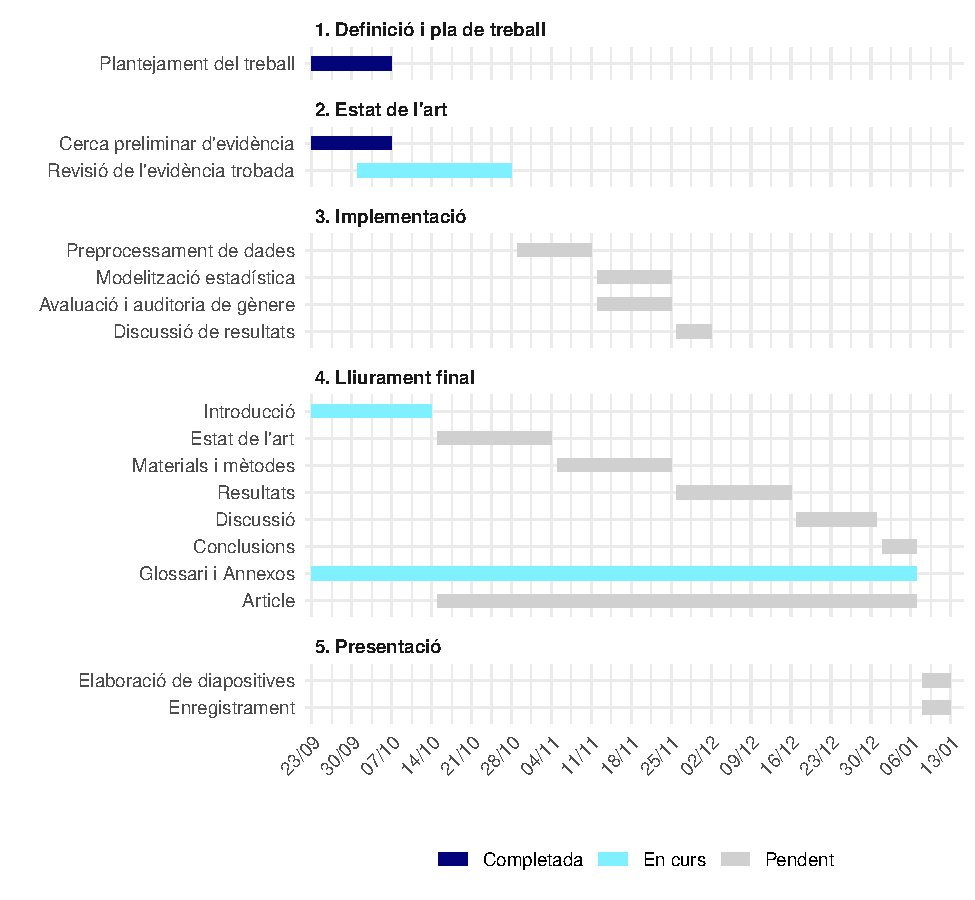
\includegraphics[width=1\linewidth]{LluisLuengo_Guillem_TFM_files/figure-latex/gantt-1} \caption{Calendari de tasques}\label{fig:gantt}
\end{figure}

\pagebreak

\subsection{Fites}\label{fites}

A la \textbf{\autoref{tab:taula1-2}} s'indiquen les fites corresponents a cada prova d'avaluació continuada (PAC).

\begin{longtable}[]{@{}lll@{}}
\caption{Fites}\label{tab:taula1-2}\tabularnewline
\toprule\noalign{}
Fita & Termini & Estat \\
\midrule\noalign{}
\endfirsthead
\toprule\noalign{}
Fita & Termini & Estat \\
\midrule\noalign{}
\endhead
\bottomrule\noalign{}
\endlastfoot
\textbf{Entrega}: PAC 1 & 7/10/26 & Completada \\
Final de la recerca bibliogràfica & 28/10/26 & En curs \\
\textbf{Entrega}: PAC 2 & 4/11/26 & Pendent \\
Final de la implementació & 25/11/26 & Pendent \\
\textbf{Entrega}: PAC 3 & 2/12/26 & Pendent \\
Cos del treball redactat & 31/12/26 & En curs \\
\textbf{Entrega}: PAC 4 i article & 7/1/27 & Pendent \\
\textbf{Entrega}: PAC 5 & 13/1/27 & Pendent \\
\end{longtable}

\subsection{Anàlisi de riscos}\label{anuxe0lisi-de-riscos}

La \textbf{\autoref{tab:taula1-3}} descriu els riscos que poden fer que la planificació no es compleixi i les accions previstes per al pla de contingència.

\begin{longtable}[]{@{}
  >{\raggedright\arraybackslash}p{(\linewidth - 6\tabcolsep) * \real{0.3014}}
  >{\raggedright\arraybackslash}p{(\linewidth - 6\tabcolsep) * \real{0.1370}}
  >{\raggedright\arraybackslash}p{(\linewidth - 6\tabcolsep) * \real{0.1781}}
  >{\raggedright\arraybackslash}p{(\linewidth - 6\tabcolsep) * \real{0.3836}}@{}}
\caption{Anàlisi de riscos}\label{tab:taula1-3}\tabularnewline
\toprule\noalign{}
\begin{minipage}[b]{\linewidth}\raggedright
Risc
\end{minipage} & \begin{minipage}[b]{\linewidth}\raggedright
Impacte
\end{minipage} & \begin{minipage}[b]{\linewidth}\raggedright
Probabilitat
\end{minipage} & \begin{minipage}[b]{\linewidth}\raggedright
Mitigació
\end{minipage} \\
\midrule\noalign{}
\endfirsthead
\toprule\noalign{}
\begin{minipage}[b]{\linewidth}\raggedright
Risc
\end{minipage} & \begin{minipage}[b]{\linewidth}\raggedright
Impacte
\end{minipage} & \begin{minipage}[b]{\linewidth}\raggedright
Probabilitat
\end{minipage} & \begin{minipage}[b]{\linewidth}\raggedright
Mitigació
\end{minipage} \\
\midrule\noalign{}
\endhead
\bottomrule\noalign{}
\endlastfoot
Abundància de registres incomplets en les dades & Alt & Alta & Imputació de valors faltants o eliminació dels registres afectats o de variables que no es considerin crítiques, segons el cas \\
Biaixos inherents a la composició del conjunt de dades & Alt & Alta & Comparació dels resultats amb l'evidència disponible i aplicació de tècniques de ponderació o remostreig \\
Desviacions del pla de treball marcat & Mitjà & Mitjana & Establiment de fites parcials per a les PAC, de manera que l'última setmana de cadascuna es pugui reservar per a la revisió o com a marge per acabar de completar les tasques pendents \\
Problemes de reproductibilitat & Mitjà & Baixa & Documentació rigorosa del codi i creació d'un repositori de GitHub que contingui tots els documents rellevants \\
\end{longtable}

\section{Resultats esperats}\label{resultats-esperats}

Al final del projecte s'obtindran els productes següents:

\begin{itemize}
\item
  Una \textbf{memòria} del treball, que contindrà la planificació, l'estat de l'art i els resultats obtinguts en el seu desenvolupament.
\item
  \textbf{Informes} de progrés per a cadascuna de les entregues de l'avaluació continuada.
\item
  Una síntesi de les troballes més rellevants en format d'\textbf{article} científic.
\item
  Una \textbf{presentació} en format virtual i les corresponents diapositives de suport.
\end{itemize}

\section{Ús responsable de la Intel·ligència Artificial}\label{uxfas-responsable-de-la-intelliguxe8ncia-artificial}

L'ús de la Intel·ligència Artificial (IA) generativa en aquest treball estarà limitat segons el que estableixen els criteris d'integritat acadèmica de la UOC. Se'n preveu l'ús en algunes tasques menors, com ara per complementar la recerca d'evidència científica, depurar codi o gestionar errors en l'exportació del document PDF final, sempre sota supervisió de l'autor.

Es declara que en cap cas s'empraran eines d'IA per a la redacció de contingut o la interpretació de resultats, ni per a cap altra tasca que pugui entrar en conflicte amb les limitacions d'un ús ètic, crític i responsable.

\chapter{Bibliografia}\label{bibliografia}

\protect\phantomsection\label{refs}
\begin{CSLReferences}{0}{1}
\bibitem[\citeproctext]{ref-tessler2026}
\CSLLeftMargin{1. }%
\CSLRightInline{Tessler J, Ahmed I, Bordoni B. Cardiac rehabilitation. Treasure Island (FL): StatPearls Publishing; 2026.}

\bibitem[\citeproctext]{ref-coutinho2025}
\CSLLeftMargin{2. }%
\CSLRightInline{Coutinho T, Khadanga S, Adedinsewo D, Barac A, Brown TM, Deaton C, et al. Cardiac rehabilitation in women: A scientific statement from the american heart association. Circulation. 2025;152:e376e390. doi:\href{https://doi.org/10.1161/cir.0000000000001379}{10.1161/cir.0000000000001379}}

\bibitem[\citeproctext]{ref-caton2024}
\CSLLeftMargin{3. }%
\CSLRightInline{Caton S, Haas C. Fairness in machine learning: A survey. ACM Computing Surveys. 2024;56:138. doi:\href{https://doi.org/10.1145/3616865}{10.1145/3616865}}

\bibitem[\citeproctext]{ref-vieli2025}
\CSLLeftMargin{4. }%
\CSLRightInline{Vieli C, Duong HP, Duc M, Carré JL, Bast JD, Girod G, et al. Functional capacity and patient-reported outcome measures after cardiac rehabilitation: A prospective study with 6-month follow-up. Swiss Medical Weekly. 2025;155:4160. doi:\href{https://doi.org/10.57187/s.4160}{10.57187/s.4160}}

\bibitem[\citeproctext]{ref-collaborators2025a}
\CSLLeftMargin{5. }%
\CSLRightInline{Collaborators G2023C of D, Naghavi M, Kyu HH, A B, Aalipour MA, Aalruz H, et al. Global burden of 292 causes of death in 204 countries and territories and 660 subnational locations, 1990{\textendash}2023: A systematic analysis for the global burden of disease study 2023. The Lancet. 2025;406:18111872. doi:\href{https://doi.org/10.1016/s0140-6736(25)01917-8}{10.1016/s0140-6736(25)01917-8}}

\bibitem[\citeproctext]{ref-abraham2021}
\CSLLeftMargin{6. }%
\CSLRightInline{Abraham LN, Sibilitz KL, Berg SK, Tang LH, Risom SS, Lindschou J, et al. Exercise{-}based cardiac rehabilitation for adults after heart valve surgery. Cochrane Database of Systematic Reviews. 2021;2021:CD010876. doi:\href{https://doi.org/10.1002/14651858.cd010876.pub3}{10.1002/14651858.cd010876.pub3}}

\bibitem[\citeproctext]{ref-dibben2023a}
\CSLLeftMargin{7. }%
\CSLRightInline{Dibben GO, Faulkner J, Oldridge N, Rees K, Thompson DR, Zwisler AD, et al. Exercise-based cardiac rehabilitation for coronary heart disease: A meta-analysis. European Heart Journal. 2023;44:452469. doi:\href{https://doi.org/10.1093/eurheartj/ehac747}{10.1093/eurheartj/ehac747}}

\bibitem[\citeproctext]{ref-firoozabadi2023}
\CSLLeftMargin{8. }%
\CSLRightInline{Firoozabadi MG, Mirzaei M, Grace SL, Vafaeinasab M, Dehghani-Tafti M, Sadeghi A, et al. Sex differences in cardiac rehabilitation barriers among non-enrollees in the context of lower gender equality: A cross-sectional study. BMC Cardiovascular Disorders. 2023;23:329. doi:\href{https://doi.org/10.1186/s12872-023-03331-7}{10.1186/s12872-023-03331-7}}

\bibitem[\citeproctext]{ref-khadanga2021}
\CSLLeftMargin{9. }%
\CSLRightInline{Khadanga S, Gaalema DE, Savage P, Ades PA. Underutilization of cardiac rehabilitation in women. Journal of Cardiopulmonary Rehabilitation and Prevention. 2021;41:207213. doi:\href{https://doi.org/10.1097/hcr.0000000000000629}{10.1097/hcr.0000000000000629}}

\bibitem[\citeproctext]{ref-hoeve2026}
\CSLLeftMargin{10. }%
\CSLRightInline{HOEVE NT, BAKKER MD, SUNAMURA M, LENNEP JERV, BOERSMA E, BERG-EMONS RJGVD. WOMEN AND MEN PROFIT EQUALLY FROM CARDIAC REHABILITATION: A SECONDARY ANALYSIS OF THE OPTICARE RCT. Journal of Rehabilitation Medicine. 2026;58:44504. doi:\href{https://doi.org/10.2340/jrm.v58.44504}{10.2340/jrm.v58.44504}}

\bibitem[\citeproctext]{ref-mcfeely2025}
\CSLLeftMargin{11. }%
\CSLRightInline{McFeely AE, Bittner VA. Sex and gender-based differences in outcomes of cardiac rehabilitation following acute myocardial infarction. Current Atherosclerosis Reports. 2025;27:109. doi:\href{https://doi.org/10.1007/s11883-025-01360-5}{10.1007/s11883-025-01360-5}}

\bibitem[\citeproctext]{ref-artiles2023}
\CSLLeftMargin{12. }%
\CSLRightInline{Artiles RF, Euler S, Auschra B, Silva HB da, Niederseer D, Schmied C, et al. Predictors of gain in exercise capacity through cardiac rehabilitation: Sex and age matter. Heart \& Lung. 2023;62:200206. doi:\href{https://doi.org/10.1016/j.hrtlng.2023.08.003}{10.1016/j.hrtlng.2023.08.003}}

\bibitem[\citeproctext]{ref-oneto2020}
\CSLLeftMargin{13. }%
\CSLRightInline{Oneto L, Chiappa S. Recent trends in learning from data, tutorials from the INNS big data and deep learning conference (INNSBDDL2019). Studies in Computational Intelligence. 2020;155196. doi:\href{https://doi.org/10.1007/978-3-030-43883-8_7}{10.1007/978-3-030-43883-8\_7}}

\bibitem[\citeproctext]{ref-criscuolo2026}
\CSLLeftMargin{14. }%
\CSLRightInline{Criscuolo C, Salnitri M, Martinenghi D. FAIR-CARE: A comparative evaluation of unfairness mitigation approaches. Information and Software Technology. 2026;189:107898. doi:\href{https://doi.org/10.1016/j.infsof.2025.107898}{10.1016/j.infsof.2025.107898}}

\bibitem[\citeproctext]{ref-fatoretto2025}
\CSLLeftMargin{15. }%
\CSLRightInline{Fatoretto MB, Özbulak G, Anjos A, Berton L. Optimizing fairness and utility in healthcare machine learning models. Applied Soft Computing. 2025;181:113426. doi:\href{https://doi.org/10.1016/j.asoc.2025.113426}{10.1016/j.asoc.2025.113426}}

\end{CSLReferences}

\newpage
\appendix

\chapter{Annex 1}\label{annex-1}

\section{Codi}\label{codi}

\begin{Shaded}
\begin{Highlighting}[]
\FunctionTok{library}\NormalTok{(knitr)}

\NormalTok{opts\_chunk}\SpecialCharTok{$}\FunctionTok{set}\NormalTok{(}\AttributeTok{echo =} \ConstantTok{FALSE}\NormalTok{,}
               \AttributeTok{warning =} \ConstantTok{FALSE}\NormalTok{,}
               \AttributeTok{message =} \ConstantTok{FALSE}\NormalTok{,}
               \AttributeTok{comment =} \StringTok{""}\NormalTok{, }
               \AttributeTok{cache =} \ConstantTok{TRUE}\NormalTok{,}
               \AttributeTok{tidy =} \ConstantTok{TRUE}\NormalTok{,}
               \AttributeTok{prompt =} \ConstantTok{FALSE}\NormalTok{,}
               \AttributeTok{tidy.opts =} \FunctionTok{list}\NormalTok{(}\AttributeTok{width.cutoff =} \DecValTok{72}\NormalTok{))}

\FunctionTok{options}\NormalTok{(}\AttributeTok{width =} \DecValTok{75}\NormalTok{)}

\FunctionTok{Sys.setlocale}\NormalTok{(}\StringTok{"LC\_TIME"}\NormalTok{, }\StringTok{"C"}\NormalTok{)}

\CommentTok{\# {-}{-}{-}{-} PAQUETS I LLIBRERIES {-}{-}{-}{-}}

\CommentTok{\#\textquotesingle{} Instal·lació de paquets}
\CommentTok{\#\textquotesingle{} }
\CommentTok{\#\textquotesingle{} @description}
\CommentTok{\#\textquotesingle{} Comrpova si els paquets d\textquotesingle{}una llista estan instal·lats al sistema. }
\CommentTok{\#\textquotesingle{} Si algun no ho està, l\textquotesingle{}instal·la automàticament.}
\CommentTok{\#\textquotesingle{}}
\CommentTok{\#\textquotesingle{} @param pkg Vector de caràcters amb els noms dels paquets.}
\CommentTok{\#\textquotesingle{}}
\CommentTok{\#\textquotesingle{} @returns No retorna cap valor.}
\CommentTok{\#\textquotesingle{} }
\CommentTok{\#\textquotesingle{} @importFrom utils install.packages}
\CommentTok{\#\textquotesingle{} @export}
\CommentTok{\#\textquotesingle{}}
\CommentTok{\#\textquotesingle{} @examples}
\CommentTok{\#\textquotesingle{} \textbackslash{}dontrun\{}
\CommentTok{\#\textquotesingle{} \# Exemple d\textquotesingle{}ús amb dades hipotètiques}
\CommentTok{\#\textquotesingle{} install\_if\_not(packages)}
\CommentTok{\#\textquotesingle{} \}}
\NormalTok{install\_if\_not }\OtherTok{\textless{}{-}} \ControlFlowTok{function}\NormalTok{(pkg) \{}
  \ControlFlowTok{for}\NormalTok{ (p }\ControlFlowTok{in}\NormalTok{ pkg) \{}
    \ControlFlowTok{if}\NormalTok{ (}\SpecialCharTok{!}\FunctionTok{requireNamespace}\NormalTok{(p, }\AttributeTok{quietly =} \ConstantTok{TRUE}\NormalTok{)) \{}
      \FunctionTok{install.packages}\NormalTok{(p, }\AttributeTok{dependencies =} \ConstantTok{TRUE}\NormalTok{)}
\NormalTok{    \}}
\NormalTok{  \}}
\NormalTok{\}}

\CommentTok{\# Llista de paquets i instal·lació}
\NormalTok{paquets }\OtherTok{\textless{}{-}} \FunctionTok{c}\NormalTok{(}\StringTok{"tidyverse"}\NormalTok{)}

\FunctionTok{install\_if\_not}\NormalTok{(paquets)}

\FunctionTok{rm}\NormalTok{(paquets)}

\CommentTok{\# Llibreries carregades}
\FunctionTok{library}\NormalTok{(tidyverse)}


\CommentTok{\# {-}{-}{-}{-} 1.6 PLANIFICACIÓ DEL TREBALL {-}{-}{-}{-}}

\CommentTok{\# Data frame de tasques}
\NormalTok{df\_gantt }\OtherTok{\textless{}{-}} \FunctionTok{data.frame}\NormalTok{(}
  \AttributeTok{Fase =} \FunctionTok{factor}\NormalTok{(}\FunctionTok{rep}\NormalTok{(}\FunctionTok{c}\NormalTok{(}
    \StringTok{"1. Definició i pla de treball"}\NormalTok{,}
    \StringTok{"2. Estat de l\textquotesingle{}art"}\NormalTok{,}
    \StringTok{"3. Implementació"}\NormalTok{,}
    \StringTok{"4. Lliurament final"}\NormalTok{,}
    \StringTok{"5. Presentació"}
\NormalTok{  ), }\AttributeTok{times =} \FunctionTok{c}\NormalTok{(}\DecValTok{1}\NormalTok{, }\DecValTok{2}\NormalTok{, }\DecValTok{4}\NormalTok{, }\DecValTok{8}\NormalTok{, }\DecValTok{2}\NormalTok{))),}
  \AttributeTok{Tasca =} \FunctionTok{c}\NormalTok{(}
    \StringTok{"Plantejament del treball"}\NormalTok{, }
    \StringTok{"Cerca preliminar d\textquotesingle{}evidència"}\NormalTok{, }
    \StringTok{"Revisió de l\textquotesingle{}evidència trobada"}\NormalTok{, }
    \StringTok{"Preprocessament de dades"}\NormalTok{, }
    \StringTok{"Modelització estadística"}\NormalTok{, }
    \StringTok{"Avaluació i auditoria de gènere"}\NormalTok{, }
    \StringTok{"Discussió de resultats"}\NormalTok{, }
    \StringTok{"Introducció"}\NormalTok{, }
    \StringTok{"Estat de l\textquotesingle{}art"}\NormalTok{, }
    \StringTok{"Materials i mètodes"}\NormalTok{, }
    \StringTok{"Resultats"}\NormalTok{, }
    \StringTok{"Discussió"}\NormalTok{, }
    \StringTok{"Conclusions"}\NormalTok{, }
    \StringTok{"Glossari i Annexos"}\NormalTok{, }
    \StringTok{"Article"}\NormalTok{, }
    \StringTok{"Elaboració de diapositives"}\NormalTok{, }
    \StringTok{"Enregistrament"}
\NormalTok{  ),}
  \AttributeTok{Objectius =} \FunctionTok{c}\NormalTok{(}
    \StringTok{""}\NormalTok{, }\StringTok{"1.1, 2.1"}\NormalTok{, }\StringTok{"1.1, 2.1"}\NormalTok{, }\StringTok{"1.2"}\NormalTok{,}
    \StringTok{"1.2"}\NormalTok{, }\StringTok{"1.2, 1.3, 2.2"}\NormalTok{, }\StringTok{"1.3, 2.2"}\NormalTok{, }\StringTok{""}\NormalTok{,}
    \StringTok{"1.1, 2.1"}\NormalTok{, }\StringTok{"1.2"}\NormalTok{, }\StringTok{"1.3, 2.2"}\NormalTok{, }\StringTok{"1.1, 1.3, 2.2"}\NormalTok{,}
    \StringTok{""}\NormalTok{, }\StringTok{""}\NormalTok{, }\StringTok{""}\NormalTok{, }\StringTok{""}\NormalTok{, }\StringTok{""}
\NormalTok{  ),}
  \AttributeTok{Inici =} \FunctionTok{as.Date}\NormalTok{(}\FunctionTok{c}\NormalTok{(}
    \StringTok{"2026{-}09{-}23"}\NormalTok{, }\StringTok{"2026{-}09{-}23"}\NormalTok{, }\StringTok{"2026{-}10{-}01"}\NormalTok{, }\StringTok{"2026{-}10{-}29"}\NormalTok{,}
    \StringTok{"2026{-}11{-}12"}\NormalTok{, }\StringTok{"2026{-}11{-}12"}\NormalTok{, }\StringTok{"2026{-}11{-}26"}\NormalTok{, }\StringTok{"2026{-}09{-}23"}\NormalTok{,}
    \StringTok{"2026{-}10{-}15"}\NormalTok{, }\StringTok{"2026{-}11{-}05"}\NormalTok{, }\StringTok{"2026{-}11{-}26"}\NormalTok{, }\StringTok{"2026{-}12{-}17"}\NormalTok{,}
    \StringTok{"2027{-}01{-}01"}\NormalTok{, }\StringTok{"2026{-}09{-}23"}\NormalTok{, }\StringTok{"2026{-}10{-}15"}\NormalTok{, }\StringTok{"2027{-}01{-}08"}\NormalTok{, }
    \StringTok{"2027{-}01{-}08"}
\NormalTok{  )),}
  \AttributeTok{Final =} \FunctionTok{as.Date}\NormalTok{(}\FunctionTok{c}\NormalTok{(}
    \StringTok{"2026{-}10{-}07"}\NormalTok{, }\StringTok{"2026{-}10{-}07"}\NormalTok{, }\StringTok{"2026{-}10{-}28"}\NormalTok{, }\StringTok{"2026{-}11{-}11"}\NormalTok{,}
    \StringTok{"2026{-}11{-}25"}\NormalTok{, }\StringTok{"2026{-}11{-}25"}\NormalTok{, }\StringTok{"2026{-}12{-}02"}\NormalTok{, }\StringTok{"2026{-}10{-}14"}\NormalTok{,}
    \StringTok{"2026{-}11{-}04"}\NormalTok{, }\StringTok{"2026{-}11{-}25"}\NormalTok{, }\StringTok{"2026{-}12{-}16"}\NormalTok{, }\StringTok{"2026{-}12{-}31"}\NormalTok{,}
    \StringTok{"2027{-}01{-}07"}\NormalTok{, }\StringTok{"2027{-}01{-}07"}\NormalTok{, }\StringTok{"2027{-}01{-}07"}\NormalTok{, }\StringTok{"2027{-}01{-}13"}\NormalTok{, }
    \StringTok{"2027{-}01{-}13"}
\NormalTok{  )),}
  \AttributeTok{Estat =} \FunctionTok{factor}\NormalTok{(}\FunctionTok{c}\NormalTok{(}
    \StringTok{"Completada"}\NormalTok{, }\StringTok{"Completada"}\NormalTok{, }\StringTok{"En curs"}\NormalTok{, }\StringTok{"Pendent"}\NormalTok{,}
    \StringTok{"Pendent"}\NormalTok{, }\StringTok{"Pendent"}\NormalTok{, }\StringTok{"Pendent"}\NormalTok{, }\StringTok{"En curs"}\NormalTok{,}
    \StringTok{"Pendent"}\NormalTok{, }\StringTok{"Pendent"}\NormalTok{, }\StringTok{"Pendent"}\NormalTok{, }\StringTok{"Pendent"}\NormalTok{,}
    \StringTok{"Pendent"}\NormalTok{, }\StringTok{"En curs"}\NormalTok{, }\StringTok{"Pendent"}\NormalTok{, }\StringTok{"Pendent"}\NormalTok{, }\StringTok{"Pendent"}
\NormalTok{  ), }\AttributeTok{levels =} \FunctionTok{c}\NormalTok{(}\StringTok{"Completada"}\NormalTok{, }\StringTok{"En curs"}\NormalTok{, }\StringTok{"Pendent"}\NormalTok{))}
\NormalTok{)}

\CommentTok{\# Tasques ordenades}
\NormalTok{df\_gantt}\SpecialCharTok{$}\NormalTok{Tasca }\OtherTok{\textless{}{-}} \FunctionTok{factor}\NormalTok{(df\_gantt}\SpecialCharTok{$}\NormalTok{Tasca, }
                         \AttributeTok{levels =} \FunctionTok{rev}\NormalTok{(}\FunctionTok{unique}\NormalTok{(df\_gantt}\SpecialCharTok{$}\NormalTok{Tasca)))}

\CommentTok{\# Dates}
\NormalTok{inici }\OtherTok{\textless{}{-}} \FunctionTok{as.Date}\NormalTok{(}\StringTok{"2026{-}09{-}23"}\NormalTok{)}
\NormalTok{final }\OtherTok{\textless{}{-}} \FunctionTok{as.Date}\NormalTok{(}\StringTok{"2027{-}01{-}13"}\NormalTok{)}

\NormalTok{dates }\OtherTok{\textless{}{-}} \FunctionTok{seq}\NormalTok{(inici, final, }\AttributeTok{by =} \StringTok{"1 week"}\NormalTok{)}

\CommentTok{\# Diagrama de Gantt}
\NormalTok{plot\_gantt }\OtherTok{\textless{}{-}} \FunctionTok{ggplot}\NormalTok{(df\_gantt, }
                     \FunctionTok{aes}\NormalTok{(}\AttributeTok{x =}\NormalTok{ Inici, }\AttributeTok{xend =}\NormalTok{ Final,}
                         \AttributeTok{y =}\NormalTok{ Tasca, }\AttributeTok{yend =}\NormalTok{ Tasca,}
                         \AttributeTok{color =}\NormalTok{ Estat)) }\SpecialCharTok{+}
  \FunctionTok{geom\_segment}\NormalTok{(}\AttributeTok{linewidth =} \DecValTok{3}\NormalTok{) }\SpecialCharTok{+}
  \FunctionTok{scale\_x\_date}\NormalTok{(}\AttributeTok{date\_labels =} \StringTok{"\%d/\%m"}\NormalTok{,}
               \AttributeTok{breaks =}\NormalTok{ dates,}
               \AttributeTok{limits =} \FunctionTok{c}\NormalTok{(inici, final),}
               \AttributeTok{expand =} \FunctionTok{expansion}\NormalTok{(}\AttributeTok{mult =} \FunctionTok{c}\NormalTok{(}\FloatTok{0.01}\NormalTok{, }\FloatTok{0.02}\NormalTok{))) }\SpecialCharTok{+}
  \FunctionTok{scale\_color\_manual}\NormalTok{(}\AttributeTok{values =} \FunctionTok{c}\NormalTok{(}\StringTok{"Completada"} \OtherTok{=} \StringTok{"\#03047a"}\NormalTok{,}
                                \StringTok{"En curs"} \OtherTok{=} \StringTok{"\#7ff0ff"}\NormalTok{,}
                                \StringTok{"Pendent"} \OtherTok{=} \StringTok{"\#d0d0d0"}\NormalTok{)) }\SpecialCharTok{+}
  \FunctionTok{facet\_wrap}\NormalTok{(}\SpecialCharTok{\textasciitilde{}}\NormalTok{ Fase, }\AttributeTok{ncol =} \DecValTok{1}\NormalTok{, }\AttributeTok{scales =} \StringTok{"free\_y"}\NormalTok{, }
             \AttributeTok{space =} \StringTok{"free\_y"}\NormalTok{) }\SpecialCharTok{+}
  \FunctionTok{theme\_minimal}\NormalTok{() }\SpecialCharTok{+}
  \FunctionTok{labs}\NormalTok{(}\AttributeTok{x =} \StringTok{""}\NormalTok{, }\AttributeTok{y =} \StringTok{""}\NormalTok{, }\AttributeTok{color =} \ConstantTok{NULL}\NormalTok{) }\SpecialCharTok{+}
  \FunctionTok{theme}\NormalTok{(}
    \AttributeTok{legend.position =} \StringTok{"bottom"}\NormalTok{,}
    \AttributeTok{axis.text.x =} \FunctionTok{element\_text}\NormalTok{(}\AttributeTok{angle =} \DecValTok{45}\NormalTok{, }\AttributeTok{hjust =} \DecValTok{1}\NormalTok{, }
                               \AttributeTok{vjust =} \DecValTok{1}\NormalTok{),}
    \AttributeTok{strip.text =} \FunctionTok{element\_text}\NormalTok{(}\AttributeTok{face =} \StringTok{"bold"}\NormalTok{, }\AttributeTok{hjust =} \DecValTok{0}\NormalTok{)}
\NormalTok{  )}

\NormalTok{plot\_gantt}

\FunctionTok{rm}\NormalTok{(inici, final, dates)}
\end{Highlighting}
\end{Shaded}


\end{document}
